\chapter{Forward Model}
\label{ch:formodel}

In this chapter we present the forward model to which we apply all our methodology on. We follow the Michelson Interferometer for Passive Atmospheric Sounding (MIPAS) handbook \cite{mipas2000handbook} and simulate data according to a cloud-free atmosphere in local thermodynamic equilibrium and assume a measurement instrument with infinite spectral resolution and no pointing errors.
\begin{figure}[ht!]
	\centering
	\input{LIMB.pdf_tex}
	\caption[Schematic of measurement and analysis geometry.]{Schematic of measurement and analysis geometry, not to scale.
		The stationary satellite, at a constant height $h_\text{sat}$ above Earth, takes $m = 41$ measurements along its line-of-sight defining by the line $\Gamma_j$.
		Each measurement has a limb height $\ell_j$, $j=1,2,\dots,m$ defined as the closest distance of $\Gamma_j$ to the Earth surface.
		Between $h_{L,0} = 7$km and $h_{L,n} = 83.3$km, the stratosphere is discretised into $n =44$ layers as illustrated by the solid green lines.}
	\label{fig:LIMB}
\end{figure}


A satellite at a constant height $h_{\text{sat}}$ points through the atmosphere (limb-sounding) and measures thermal radiation of gas molecules along its straight line of sight $\Gamma_j$, see  Figure~\ref{fig:LIMB}.
One measurement of the thermal radiation of one specific molecule, in our case ozone denoted by the ozone volume mixing ratio $x(r)$ at distance $r$ from the satellite, at the wave number $\nu$ is given by the path integral
\begin{align}
	\label{eq:RTE} 
	y_j =   \int_{\Gamma_j}  B(\nu,T) k(\nu, T)   \frac{p(T)}{k_{\text{B}} T(r)}  x(r)  \tau(r) \text{d}r + \eta_j \, \\
	\tau(r) = \exp{ \Bigl\{ - \int^{r}_{r_\text{obs}}  k(\nu, T)   \frac{p(T)}{k_B T(r^{\prime})}  x(r^{\prime}) \text{d}r^{\prime} \Bigr\} } \, ,\label{eq:absRTE} 
\end{align}
which is the radiative transfer equation (RTE)~\cite{mipas2000handbook}.
For more information on the processes within the atmosphere for ozone we refer to \cite{Lee2020NightOzone}.
We define a tangent height $h_{\ell_j}$ and $\Gamma_j$ for each $j=1,2,\ldots,m$, so that the data vector $\bm{y} \in \mathbb{R}^m$ including some noise $\eta_j$.
Within the atmosphere the number density $p(T) / (k_{\text{B}} T(r))$ of molecules is dependent on the pressure $p(T)$, the temperature $T(r)$, and the Boltzmann constant $k_{\text{B}}$.
The factor $\tau(r)\leq 1$ accounts for re-absorption of the radiation along the line-of-sight, which makes the RTE non-linear.
The absorption constant
\begin{align}
	k(\nu, T) = L(\nu, T_{\text{ref}}) \frac{Q(T_{\text{ref}})}{Q(T)} \frac{ \exp{\{ - c_2 E^{\prime \prime} / T\}} }{\exp{\{ - c_2 E^{\prime \prime} / T_{\text{ref}} \}}} \frac{ 1- \exp{\{ - c_2 \nu  / T \}} }{1 - \exp{\{ - c_2 \nu / T_{\text{ref}} \}}}
\end{align}
is dependent on the line intensity $L(\nu, T_{\text{ref}})$ at reference temperature $T_{\text{ref}} =296K $, the lower-state energy of the transition $ E^{\prime \prime} $, the second radiation constant $c2=1.4387769\text{cmK}$ all provided by the HITRAN database \cite{gordon2022hitran2020}.
Since we assume that the measurement deceive has negligible frequency window we neglect line broadening around $\nu_0$ for the calculations of $L(\nu, T_{\text{ref}})$, which would normally be modelled as a convolution of the normalised Lorentz profile (collisional/pressure broadening) and the normalised Doppler (thermal broadening) profile \cite{}.
Additionally, since we target one specific molecule, we simplify the calculation of $k(\nu, T)$, which usually the sum the individual absorption constants for each targeted molecule weighted by the respective volume mixing ratio \cite{}.
The total internal partition function for the lower-state energy is given as:
\begin{align}
	Q(T )= g^{\prime \prime} \exp{\{ - \frac{ c_2 E^{\prime \prime} }{T}\}} \, ,
\end{align}
with the statistical weight $ g^{\prime \prime}$ (also called the degeneracy factor) accounting for the molecules non-rotational and rotational energy states, see \cite{vsimevckova2006einstein}.
Under the assumption of local thermodynamic equilibrium (LTE) the black body radiation acts as a source function
\begin{align}
	B(\nu,T)   = \frac{2 h c^2 \nu^3}{\exp{\{\frac{hc\nu}{k_B T}\}}-1}\, ,
\end{align}
with Planck's constant $h$ and velocity of light $c$ \cite{}.
For fundamentals on the Radiative transfer equation we recommend \cite[Chapter 1]{rybicki2000rte}, and for a more comprehensive model we refer to \cite{read2006forwardModel}

To enable matrix-vector multiplication, we discretise the atmosphere in $n$ layers, where the $i^\text{th}$ layer is defined by two spheres of radii $h_{L,i-1} < h_{L,i}$, for $i = 1, \dots, n$, with $h_{L,0}$ and $h_{L,n} $.
Then we can discretise the ozone, pressure and temperature profiles as a function of height, where in between the heights $h_{L,i-1}$ and $h_{L,i}$, each of the ozone concentration $x_{i}$, the pressure $p_{i}$, the temperature $T_{i}$, as well as all other height dependent parameters are assumed to be constant.
Above $h_{L, n}$ and below $h_{L,0} $, the ozone concentration is set to zero, so no signal can be obtained.
Depending on the parameter of interest, which is either the ozone volume mixing ratio $\bm{x} =\{x_1,x_2,\ldots,x_n\} \in \mathbb{R}^{n}$ or the fraction of pressure and temperature $\bm{p/T}= \{p_1/T_1,p_2/T_2,\ldots,p_n/T_n\} \in \mathbb{R}^{n} $
we rewrite the integral in Eq.~\eqref{eq:RTE} for one noise free measurement using the trapezoidal rule as a vector-vector multiplication $\bm{A_{j}}(\bm{x},  \bm{p},\bm{T}) \, \bm{x} $ or $\bm{A_{j}}(\bm{x},  \bm{p},\bm{T}) \, \bm{p}/ \bm{T} $, where the non-linear absorption $\tau(r)$ is included in $\bm{A_{j}}(\bm{x},  \bm{p},\bm{T}) \in \mathbb{R}^{n}$ which is the $j$-th row of the matrix $\bm{A}(\bm{x},  \bm{p},\bm{T})$.
Then given a noise vector $\bm{\eta} \in \mathbb{R}^{m}$ the data vector
\begin{align}
	\bm{y} = \bm{A}_{NL} \, \bm{x} + \bm{\eta}= \bm{A}_{NL} \,
	\frac{ \bm{p}}{\bm{T}} + \bm{\eta} \, 
\end{align}
is based on a matrix-vector multiplication.
Here we define the non-linear forward model matrix as $\bm{A}_{NL} \coloneqq \bm{A}(\bm{x},  \bm{p},\bm{T})   \in \mathbb{R}^{m \times n}$ for simplicity so that $\bm{A}_{NL}\bm{x}$ or $\bm{A}_{NL}\bm{p}/\bm{T}$ implies the construction of $\bm{A}_{NL}$ and similarly for $\bm{A}_L$, which denotes the linear forward model matrix and neglects abortion (e.g. set $\tau = 1$ in Eq.~\eqref{eq:absRTE}).
Further, we classify the inverse problem as weakly non-linear, see e.g. Fig. \ref{fig:MapAsses}, as neglecting the absorption changes the measurements only slightly.



\section{Singular value decomposition of linear forward model matrix}
Prior to simulating some data, we provide a quick and intuitive way of how we can asses which measurement setup is effective, how much information passed through the forward model and how the signal to noise ratio affects that information.
One way of doing this is via a singular value decomposition (SVD) of the forward model matrix
\begin{align}
	\bm{A} = \sum_{i =1}^{r} \bm{u}_i  \sigma_i \bm{v}^T_i = \bm{U} \bm{\Sigma} \bm{V}^T
\end{align}
where $r = \min\{m,n\}$ for a forward model $\bm{A} \in \mathbb{R}^{m \times n}$.
Consider $\bm{A}\bm{x}$, then the SVD gives us information of how information is picked up from the parameter space by the forward model, described through the right singular values $\bm{v}_i$.
Then the singular values $\sigma_i $, ordered in size from the largest $\sigma_1$ to the smallest $\sigma_{r}$, weight that information and the left singular values $\bm{u}_i$ project onto the data space.
So if the right singular vectors are flat in heigh altitudes the forward model does not pick up any structure of the parameter in that region.
Further for very small singular values $\sigma_i \ll \sigma_1/\text{SNR}$ below the root mean square (rms) noise level or the noise standard deviation (std.), we can introduce an effective rank $r_{\text{eff}} \leq r$.
Then information of parameter space spanned by $ \{\bm{v}_{r_{\text{eff}} +1}, \dots ,\bm{v}_r \}$ is not passed through the forward model and the data is noise dominated noise dominated for the corresponding data space, see Figure \ref{fig:nullSpac}.
This is based on the rough assumption that if we define the signal to noise ratio (SNR) as
\begin{align}
	\text{SNR} \coloneqq \frac{\max(y)}{\text{std. noise}} = \frac{\text{peak signal}}{\text{rms noise}}
\end{align}
then the maximum singular value $\max(y) \approx \sigma_1$ and the information transmitted through the forward model corresponds roughly to the singular values $s_i \gtrsim \max(y)/ \text{SNR}$.
See \cite{tan2016LecNot} for a more comprehensive analysis.

\begin{figure}[ht!]
	\centering
	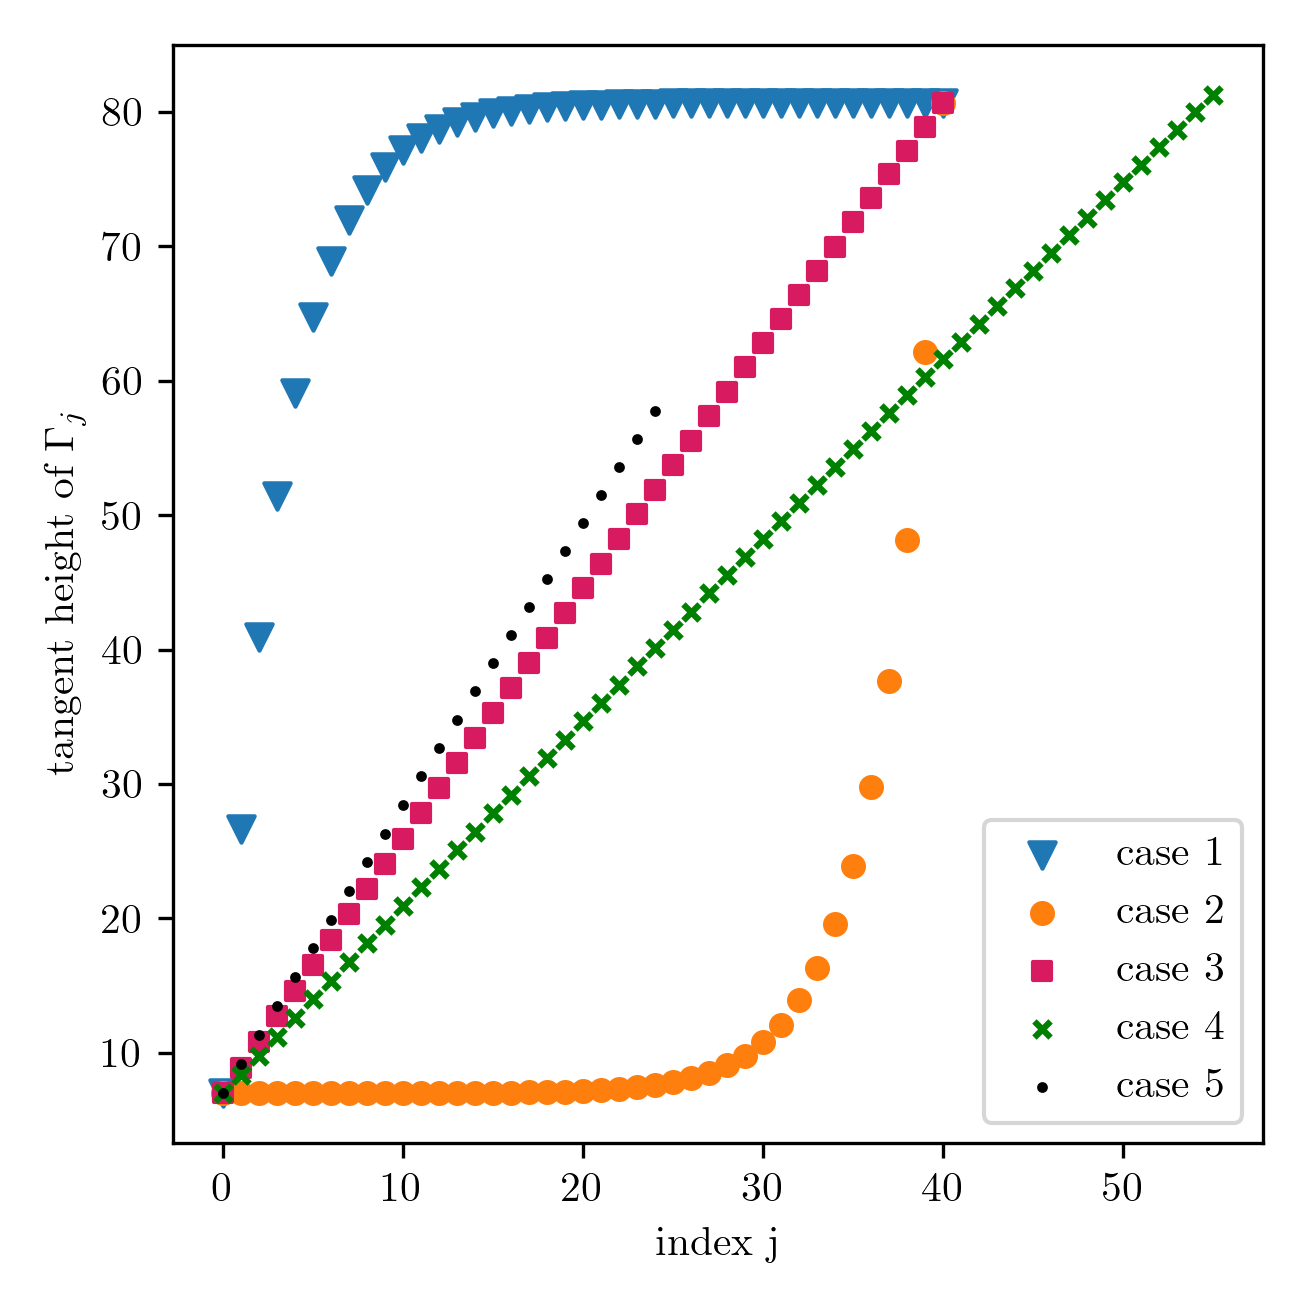
\includegraphics{MeasTangHeight.png}
	\caption[Tangent heights for different sequence of measurements.]{We plot the tangent heights for different cases of measurements.}
	\label{fig:TangHCases}
\end{figure}
\begin{figure}[ht!]
	\centering
	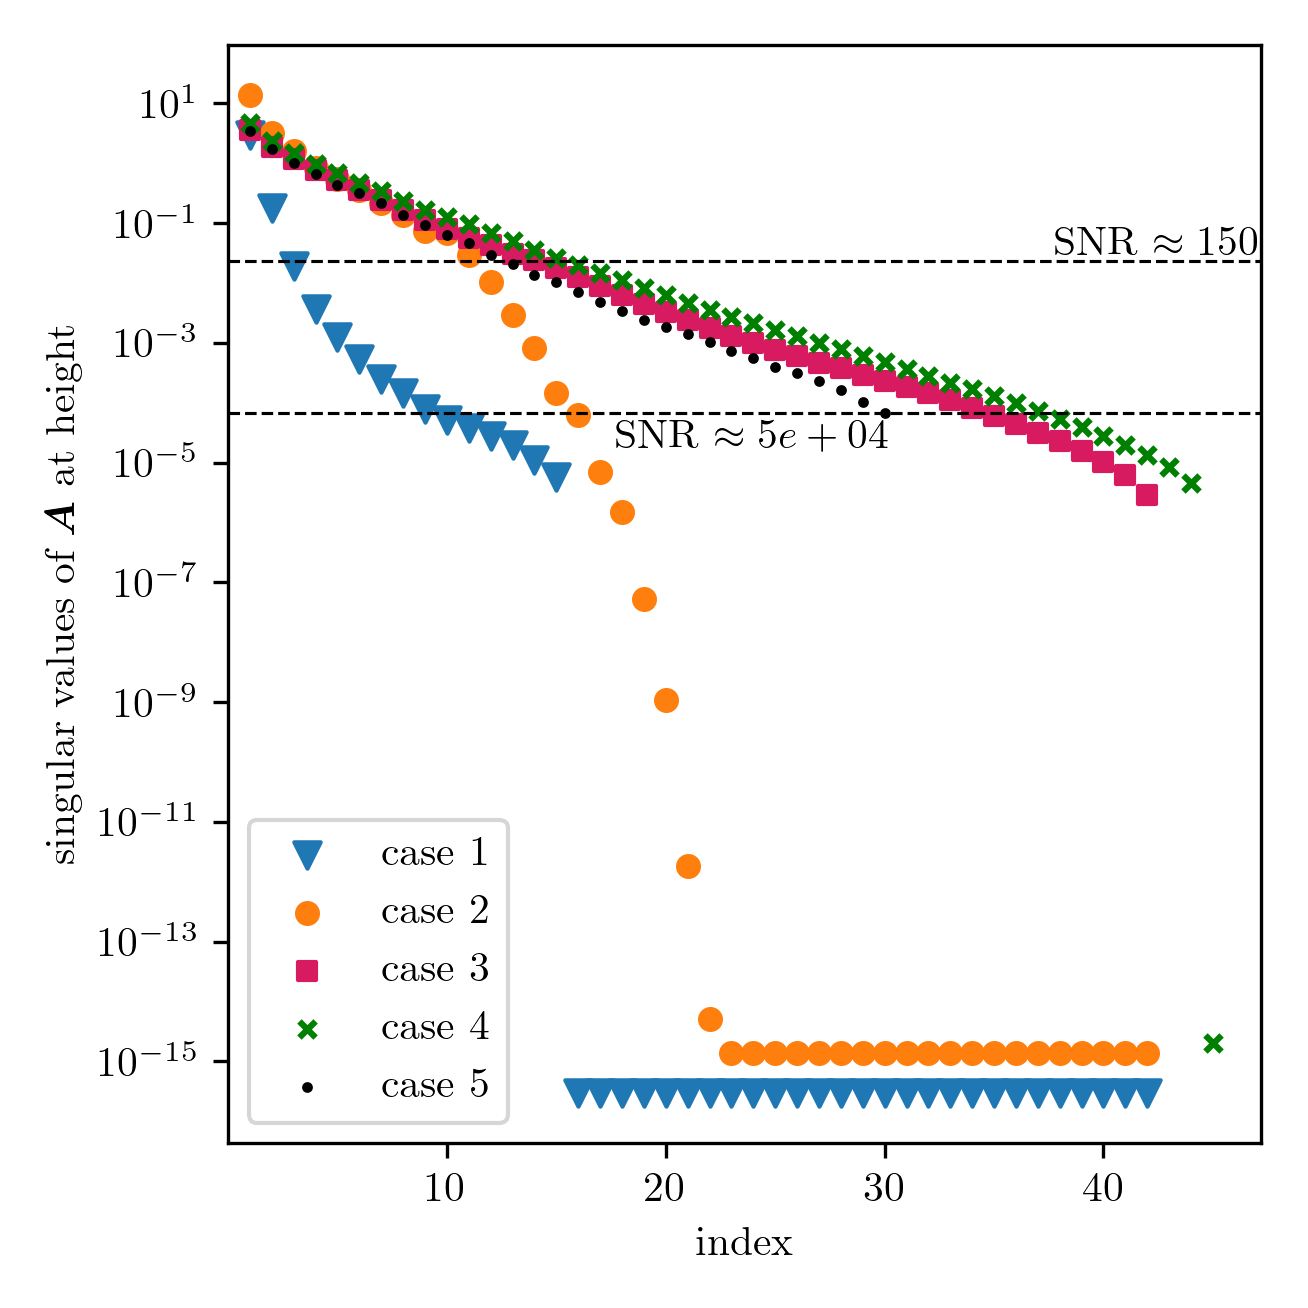
\includegraphics{SingValA.png}
	\caption[Singular values of linear forward model matrix for different sequences of measurements.]{We plot the singular values of linear forward model matrix for different sequences of measurements.
		The corresponding tangent heights of the different cases are plotted in Fig. \ref{fig:TangHCases}. We include an approximate for the disiered Signal to noise ratio if $s_1 \approx max(\bm{y}) $ the signal.}
	\label{fig:SingA}
\end{figure}
Next we analyse the singular values for a few different measurement scenarios, to see which of those measurement cases is most effective.
Our objective is to measure ozone $\bm{x}$ so our forward model $\bm{A}$ includes pressure and temperature.
The information captured by the forward model is influence by the in height exponentially decreasing pressure.
Hence we test different measurement scenarios, where we either measure at equidistance tangent heights or collect more data from high signal regions at low attitudes, where the pressure is high and the noise low, or at high altitudes, where the pressure is low and the data is noise dominated.
We start with case 3 in Fig. \ref{fig:TangHCases} where the pointing accuracy of $150\text{arc sec}$ was given to us by the team of the University of New South Wales Canberra Space \cite{CubeSatInternal}.
The pointing accuracies determines how well the satellite can point in a certain direction and hence roughly the number of measurements we can take.
The corresponding singular values are plotted in Fig. \ref{fig:SingA}, which do decrease linear in log-space and about 10-15 singular values lay above the SNR.
In comparison if we measure a lot of times in regions where we the data is noise dominated (high altitude), case 1, we do obtain more information since the singular values decrease rapidly.
Measuring lots of times at low altitudes, where the data is informative, and less at higher altitudes, case 2, does not seem optimal as the we get one larger singular values but the singular values decrease faster compared to case 3.
Now if we have double the number of equidistance measurement, case 4, we do get slightly larger singular values but not significantly that is would be worth the engineering effort required to achieve that.
Since we want to measure most efficiently and with low effort we choose a measurement set with equidistance tangent height.
By exploratory analysis we find that we can tolerate a slightly larger distance, case 5, between tangent height than required by \cite{CubeSatInternal}.
We choose the measurement setup so that we obtain enough data points in regions with high signal and stop measuring when the signal is too noisy.
We like to note that if would want to obtain all information provided by the forward model we would need a signal to noise ratio of roughly $10^16$, which seems technically impossible.

In principle we show that it does not depend on how one measures, one can not get more information by measuring more in regions where the information content is low or high \cite{livesey2006retrieval}.
This contradicts with the current measurement setup on the AURA MLS \cite{}, which reports high noise in lower atmospheric regions, due thermal radiation from the earth, and measures more in those regions.


\begin{figure}[ht!]
	\centering
	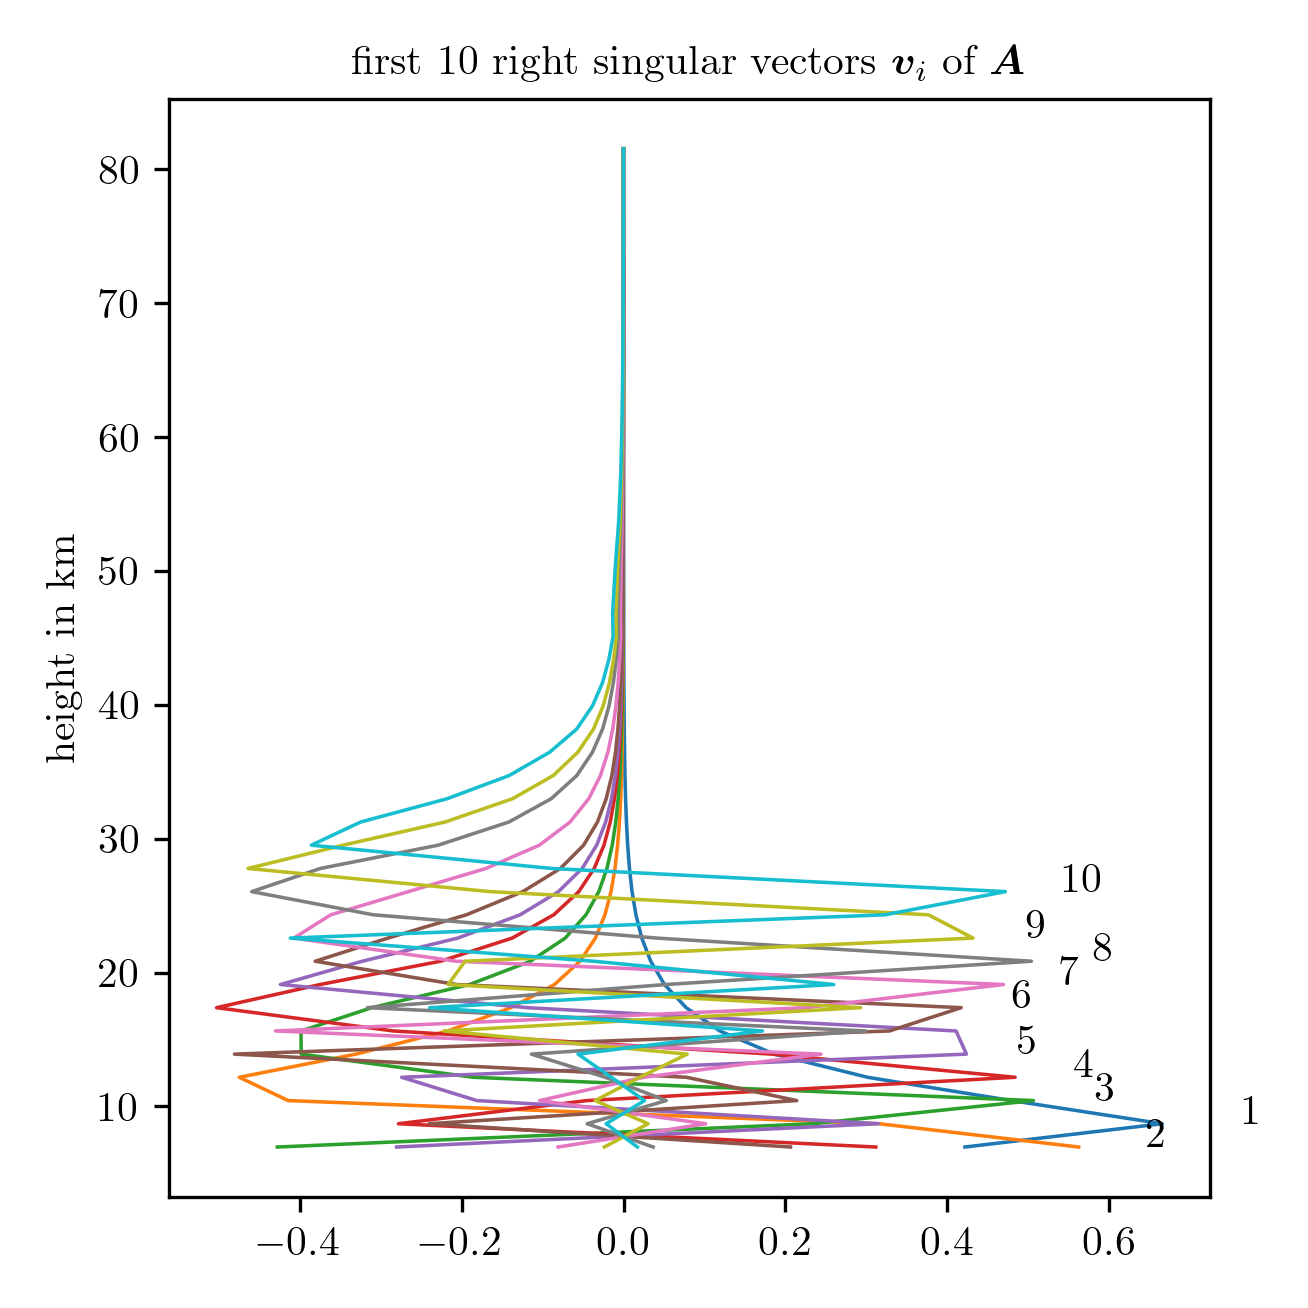
\includegraphics{SingVecA.png}
	\caption[Left singular vectors of forward model matrix for one sequence of measurements.]{We plot the first 20 left singular vectors of forward model matrix for case 5 sequence of measurements, see Fig. \ref{fig:SingA}.}
	\label{fig:SingVecA}
\end{figure}
\begin{figure}[ht!]
	\centering
	%\includegraphics{}
	\caption[]{}
	\label{fig:nullSpace}
\end{figure}
Consequently we proceed with case 5 and plot the parameter space of the model for the first 20 of 25 or so right singular vectors in Fig. \ref{fig:SingVecA}
We observe that we do not pick up structures above 60km.
The last 5 right singular vectors (null space) include structures above 60 km and hence our model is not sensitive to those.

 Says that the instrument spents more time in lower regions, this does not increase perfomance !!!


This says that ozone is the main emitter around 240 Ghz \cite[34]{livesey2008ozonecarbonmono}

We dont csider emittsion from other source wjhich might skew the measuremtns as well.
